\subsection{Ondas estacionárias de som em um gás nobre
desconhecido}

Nessa parte da prática, também iremos utilizar o Tubo de Kundt, que agora, está preenchido com um gás desconhecido. Queremos encontrar a velocidade do som nesse gás desconhecido, para então, descobrir qual foi o gás utilizado. O alto-falante será excitado através de um gerador de voltagem harmônico com frequência \textit{f} fixa. 

\begin{figure}[H]
  \centering
  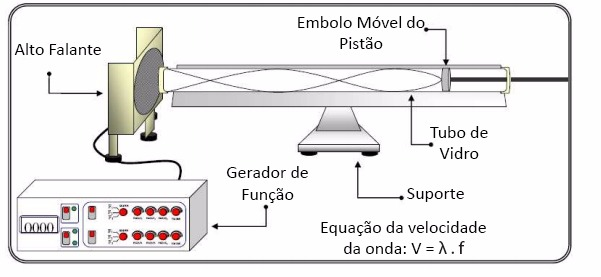
\includegraphics[scale=0.7
  ]{images/TKundt.jpg}
  \caption{Esquema do Tubo de Kundt}
\end{figure}

Nesse experimento, manteremos uma frequência \textit{f} fixa e vamos variar o comprimento L da coluna de gás até obtermos o primeiro harmônico. 

\begin{figure}[H]
  \centering
  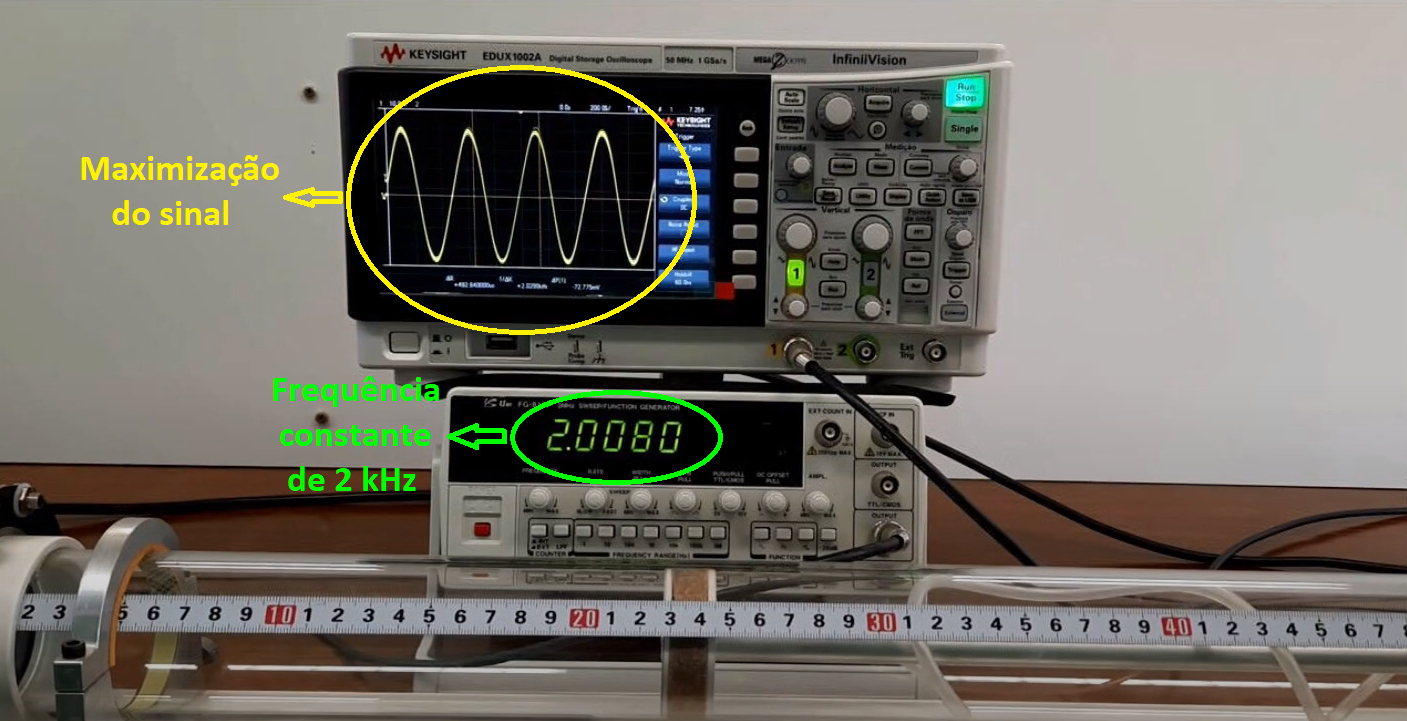
\includegraphics[scale=0.48]{images/Exp1.png}
  \caption{Frequência \textit{f} fixada nesse experimento}
\end{figure}

\begin{figure}[H]
  \centering
  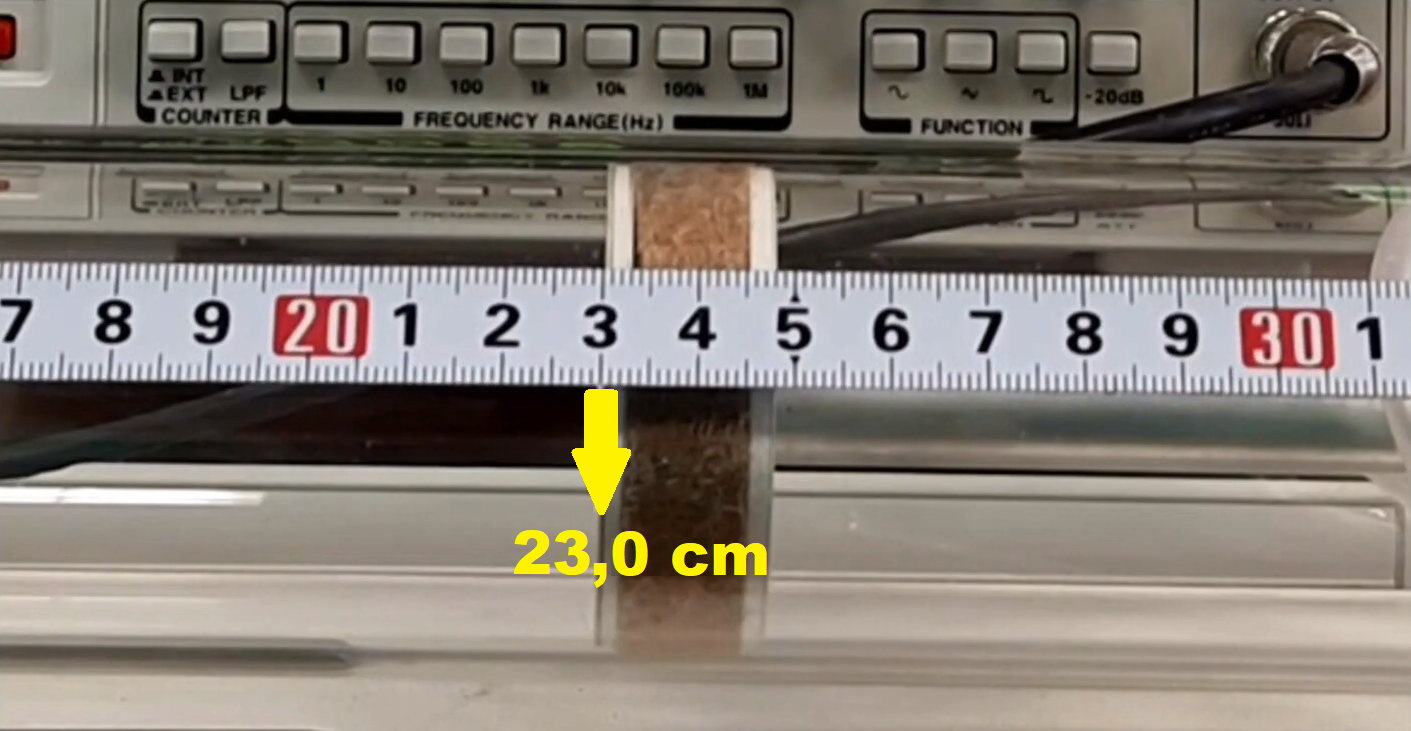
\includegraphics[scale=0.48]{images/L (23cm).png}
  \caption{Comprimento L da coluna de gás para o primeiro harmônico}
\end{figure}

Desse fato, podemos perceber que a relação entre a frequência do primeiro harmônico $f_1$, o comprimento L e a velocidade do som no gás é dada por:

\[ v = 2 \cdot L \cdot f\]

Assim, poderemos determinar a velocidade do som no gás e descobrir qual gás é esse, consultando literaturas.
